\chapter{JavaScript-ohjelman muuttaminen staattisesti tyyppitarkastetuksi}

\section{Tyyppiannotaatiot}

Tyyppijärjestelmä voi päätellä muuttujan sallitun tyypin automaattisesti
päättelemällä tai kieleen sisältyvien eksplisiittisten tyyppimäärittelyjen
perusteella. Kaikki kolme tässä esiteltyä JavaScriptin staattiseen
tyyppitarkastukseen tarkoitettua työkalua päättelevät muuttujien tyyppejä automaattisesti, mutta vaativat
myös eksplisiittisiä määrityksiä paikoitellen. 

\begin{minipage}{\linewidth}
Closure-kääntäjä lukee
tyyppimääritykset JSDoc-tyylisistä dokumentaatiokommenteista \cite{annotatingJSforClosure}.
\begin{lstlisting}[caption={Esimerkki Closure-annotaatiosta funktiolle},label={lst:ostoskorin_hinta_clojure}]
/**
* @param {!Array<Ostos>} ostokset
* @return {number} Ostosten yhteenlaskettu hinta
*/
function ostoskorinHinta(ostokset) {
  let summa = 0;
  for (const ostos of ostokset) summa += ostos.hinta;
  return summa;
}
\end{lstlisting}
\end{minipage}
TypeScript ja Flow puolestaan jatkavat ECMA-262 -spesifikaatiota erityisellä syntaksilla
tyyppien eksplisiittistä määrittämistä varten. 

\begin{minipage}{\linewidth}
\begin{lstlisting}[caption={Esimerkki Flow tai TypeScript annotaatiosta funktiolle},label={lst:ostoskorin_hinta_flow}]
function ostoskorinHinta(ostokset: Ostos[]): number {
\end{lstlisting}
\end{minipage}

Flow ja TypeScript -esimerkeissä tyyppiannotaatiot ovat osana koodia, mikä
tekee ohjelmasta yhteensopimattoman tavallisen JavaScriptin kanssa. Ohjelma
on käännettävä JavaScriptiksi ennen suorittamista, eikä annotaatioiden
syntaksi ja merkitys ole suoraan selvä JavaScript-ohjelmoijalle. 

Closuren annotaatiot on sijoitettu kommentteihin, joten niillä ei ole
ajonaikaista vaikutusta ja ohjelma on täten sellaisenaan hyväksyttävää
JavaScriptiä. Toisaalta kommentit voivat olla hankala ja runsassanainen
formaatti monimutkaisille tyyppiannotaatioille, mikä kasvattaa niiden
kirjoittamiseen vaadittua työmäärää \cite{TypeScriptSpec}\cite{TypeScriptatBuild}.

\begin{minipage}{\linewidth}
Aiemmassa esimerkissä esitelty tyyppi \inlinecode{Ostos} pitäisi
määritellä Closurea varten muiden annotaatioiden tapaan dokumentaatiokommentteja käyttäen:
\begin{lstlisting}[label={lst:closure_typedef}]
/**
* @typedef {{
*   hinta: number
* }}
*/
let Ostos;
\end{lstlisting}
\end{minipage}

TypeScript ja Flow tarjoavat vastaavan käännösaikaisen tyypin (type alias)
määrittelyyn tiiviimmällä syntaksilla \cite{TypeScriptSpec}:

\begin{minipage}{\linewidth}
\begin{lstlisting}[label={lst:ts_flow_type_alias}]
type Ostos = {
  hinta: number;
};
\end{lstlisting}
\end{minipage}
Tällainen tyypin määritteleminen vaikuttaa ainoastaan käännösvaiheen
tyyppitarkastukseen, eikä määrittely tuota tietorakenteita tai muuta
sisältöä suoritettavaan JavaScript-ohjelmaan.

\section{Ohjelman kääntäminen ennen suorittamista}

JavaScript koodi tulkataan tai käännetään tyypillisesti suorittamisen
yhteydessä, selaimesta tai muusta suoritusympäristöstä löytyvän ”moottorin”
toimesta. EcmaScript standardin mukaista koodia suorittamaan suunnitellut
moottorit, kuten V8 tai SpiderMonkey, eivät kuitenkaan osaa käsitellä
TypeScript- tai Flow-annotaatioilla merkattua koodia. Näinollen TypeScript-
tai Flow-annotoitu koodi on välttämätöntä kääntää muotoon jossa
annotaatiot on poistettu ja jäljellä on enää standardinmukainen JavaScript.
Koska JavaScriptin käyttäminen ei normaalisti vaadi erillistä
käännösvaihetta, useissa projekteissa ei ole sellaista käytetty. Koodin
minimointi ja muu optimointi on ollut parhaiden käytäntöjen mukaista jo
tovin, mutta tällaiset koodinkäsittelyt tehdään yleensä vasta ennen koodin
julkaisua. Kehittäjät ovat tavanomaisesti voineet suorittaa kirjoittamansa
JavaScriptin sellaisenaan kehitysympäristössä. Käännösvaiheen aikavaatimus
pyritään luonnollisesti pitämään mahdollisimman pienenä, mutta se on silti
projektin monimutkaisuuteen ja kehitysnopeuteen vaikuttava tekijä joka
työkalun käyttöönotossa tulee huomioida.

\begin{figure}
\centering
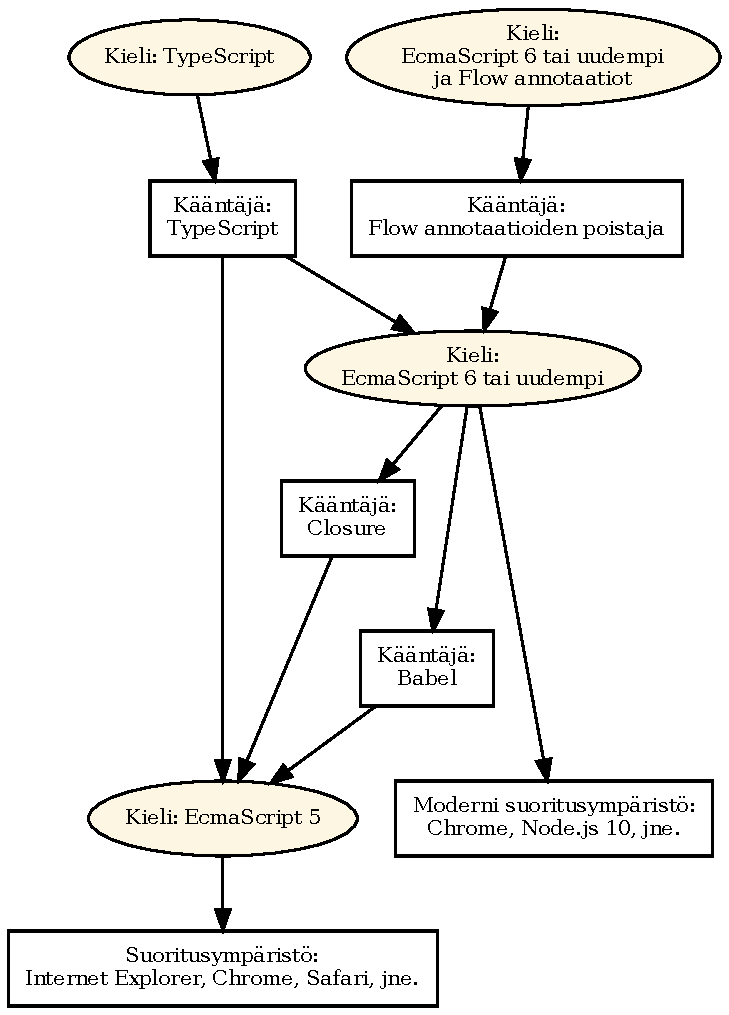
\includegraphics[width=0.6\textwidth]{images/compilation.pdf}
\caption{Käännösprosessi}
\end{figure}

\section{Työkalun vaiheittainen käyttöönotto}

Kun kyseessä on jo olemassa olevan kielen, JavaScriptin, muuttaminen
staattisesti tyyppitarkastetuksi, eräs merkittävä tekijä on että suuria
määriä koodia voidaan jo olla kehitetty alkuperäisellä kielellä ilman
tyyppitarkastuksista huolehtimista. Näin ollen tärkeäksi tekijäksi nousee
vaiheittainen käyttöönotto. On tärkeää että olemassa olevaa annotoimatonta
koodipohjaa voi yhä käyttää uuden, staattisesti tyyppitarkastetun koodin
kanssa. Flow-tarkastukset lisätään olemassa olevaan JavaScript-koodiin
erityisellä kommentilla. JavaScriptin muuttamisessa TypeScriptiksi riittää
yleensä tiedostopäätteen muuttaminen. Closure toimii ilman erillistä
muunnosta, kunhan tarvittava määrä dokumentaatiopohjaisia tyyppimäärittelyitä
on annettu. Sekä Flow että TypeScript tarjoavat myös erityisen
yleisviittaustyypin Any, jota voi käyttää kuvaamaan mitä tahansa JavaScript
arvoa \cite{TypeScriptSpec}. Any tyyppiseen muuttujaan voidaan asettaa mikä
tahansa arvo ja Any tyyppinen arvo voidaan asettaa mihin tahansa muuttujaan
tai funktioparametriin. Any tyypin avulla muuten staattisesti tyypitetyssä
ohjelmassa voidaan ohittaa käännösaikainen tyyppien tarkistaminen sellaisten
koodin osien kohdalla joiden ajonaikaista arvoa olisi muuten vaikea tai
mahdotonta määritellä käännösaikana.